% Created 2017-10-30 Mon 15:21
% Intended LaTeX compiler: pdflatex
\documentclass[11pt]{article}
\usepackage[utf8]{inputenc}
\usepackage[T1]{fontenc}
\usepackage{graphicx}
\usepackage{grffile}
\usepackage{longtable}
\usepackage{wrapfig}
\usepackage{rotating}
\usepackage[normalem]{ulem}
\usepackage{amsmath}
\usepackage{textcomp}
\usepackage{amssymb}
\usepackage{capt-of}
\usepackage{hyperref}
\usepackage{minted}
\usepackage{pdflscape}
\author{Willian Ver Valen Paiva}
\date{}
\title{Capstone Proposal}
\hypersetup{
 pdfauthor={Willian Ver Valen Paiva},
 pdftitle={Capstone Proposal},
 pdfkeywords={},
 pdfsubject={},
 pdfcreator={Emacs 27.0.50 (Org mode 9.1.1)}, 
 pdflang={English}}
\begin{document}

\maketitle

\section{Machine Learning Engineer Nanodegree}
\label{sec:org76d5988}
\subsection{Domain Background}
\label{sec:org0a4a041}

For a long time work in facial recognition has being done and one of the key
points of this work is the face alignment as it poses its own challenge.
And the main tool used for the job is OpenCV which is used with DLIB to
recognize Facial landmarks.

The automatic recognition of landmarks is essential to be able to classify
facial expressions, or face tracking, face animation, and even 3D face
modeling.

For example to classify facial expressions it is necessary to classify
Facial Action Units also known as FACS \cite{ekman1977facial}, which in turn
needs a proper face alignment.

As one of my main projects today is to create a model capable to recognize
facial expression of pain, this subject comes to be perfect as it cover a
personal necessity and brings a good subject to work and learn.


\subsection{Problem Statement}
\label{sec:orgc779fb9}
The problem of face alignment is among the most popular in the field of
computer vision and today we have many different implementations to
automatically recognize facial landmarks on images.
The most known is the Active Appearance Model (AAM)
\cite{edwards1998face,matthews2004active}.

But today we also some good results using Deep learning to achieve the
results for example the work done by Adrian Bulat on recognizing 3D facial
landmarks \cite{bulat2017far} that shows remarkable results it is implemented in torch.
a framework for \textbf{LUA}.

In resume to find an implementations on Tensorflow is not that easy. As most of the
works done on the subject is heavily dependent of DLIB to recognize the
landmarks. and as of today Tensorflow is a library that is on the rise and having such a
tool would be a plus and a entry point for more detailed facial expressions.

So for that reason I propose for this project to create a Deep Neural Network to
tackle such subject and have a model with better of equivalent performance of
the DLIB counter part on Tensorflow.

As the DLIB model has difficulty on recognizing points on faces by the side
view. 


\subsection{Dataset and Inputs}
\label{sec:org7053fa3}

When looking for a data set for facial landmarks is possible to find many of
them example:

\begin{itemize}
\item AFLW \cite{sagonas2013300}
\item Cohn-Kanade AU-Coded Expression Database \cite{cohn1999cohn}
\item Affectiva-mit facial expression dataset (am-fed) \cite{mcduff2013affectiva}
\end{itemize}

But for this capstone project I propose to use the MUCT Face Database
\cite{Milborrow10}, this dataset consists of pictures taken from 276 subjects
using 5 cameras in different angles an light conditions like the image below:

\begin{figure}[htbp]
\centering
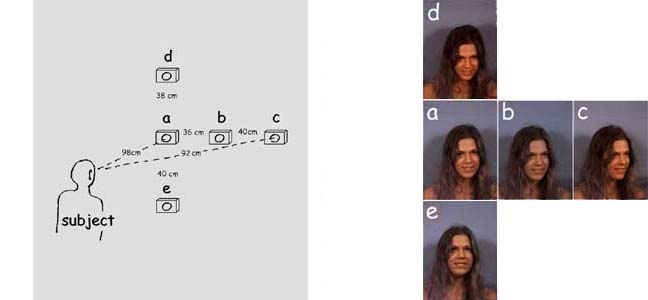
\includegraphics[width=.9\linewidth]{./images/muct-views-lores.jpg}
\caption{There is no images on the left but they cam be reproduced by mirroring the right side}
\end{figure}

Each picture is coded with 76 facial landmark like:
\begin{center}
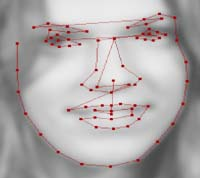
\includegraphics[width=.9\linewidth]{./images/landmarks.jpg}
\end{center}

The choice of this dataset is made because it has a reasonable size to train
on personal computers and moreover it has large room for data augmentation
if necessary
The focus on using this data set is that it provides data
to have a better result when the face is in the side view.


The dataset is public available via github on the following link
\url{https://github.com/StephenMilborrow/muct}

\subsection{Solution Statement}
\label{sec:org9c1b393}

What I am hoping to achieve from this project is to have a pre trained model that is capable
of marking images properly with landmarks using a Tensorflow  backend, obtaining 
achieve results at least as good as the DLIB model, for that I will be using
our own Convolutional Neural Networks and pre-trained networks to find the best
result for the task.

\subsection{Evaluation and Metrics}
\label{sec:orgc329deb}

As the problem consists on a regression model I believe that for the
evaluation of the results I could use the accuracy calculated by using one
of the regression functions R-squared OR mean-squared.

\subsection{Project Design}
\label{sec:org3b4fa7e}

To solve such a problem I will begin from the point of training my own model
using Convolutional Neural Networks and use it as the starting point and compare
the results with other models using transfer learning like inception v3 , resnet, vgg16.

The main idea here is to create a model with 152 regression outputs giving
the respective X and Y of each point.

In case the transfer learning don't give good results another approach would
be go up on the pre-trained model and get more fine tuning.
By using the option include\(_{\text{top}}\) from keras and augment the number of layers
that will be trained. What would increase the time of training but give better results.



\bibliographystyle{unsrt}
\bibliography{repport}
\end{document}